%Copyright 2014 Jean-Philippe Eisenbarth
%This program is free software: you can 
%redistribute it and/or modify it under the terms of the GNU General Public 
%License as published by the Free Software Foundation, either version 3 of the 
%License, or (at your option) any later version.
%This program is distributed in the hope that it will be useful,but WITHOUT ANY 
%WARRANTY; without even the implied warranty of MERCHANTABILITY or FITNESS FOR A 
%PARTICULAR PURPOSE. See the GNU General Public License for more details.
%You should have received a copy of the GNU General Public License along with 
%this program.  If not, see <http://www.gnu.org/licenses/>.

%Based on the code of Yiannis Lazarides
%http://tex.stackexchange.com/questions/42602/software-requirements-specification-with-latex
%http://tex.stackexchange.com/users/963/yiannis-lazarides
%Also based on the template of Karl E. Wiegers
%http://www.se.rit.edu/~emad/teaching/slides/srs_template_sep14.pdf
%http://karlwiegers.com
\documentclass{scrreprt}
\usepackage{listings}
\usepackage{underscore}
\usepackage[bookmarks=true]{hyperref}
\usepackage[utf8]{inputenc}
\usepackage[english]{babel}
\usepackage{graphicx}
\hypersetup{
    pdftitle={Software Requirement Specification},    % title
    pdfauthor={Jean-Philippe Eisenbarth},                     % author
    pdfsubject={TeX and LaTeX},                        % subject of the document
    pdfkeywords={TeX, LaTeX, graphics, images}, % list of keywords
    colorlinks=true,       % false: boxed links; true: colored links
    linkcolor=blue,       % color of internal links
    citecolor=black,       % color of links to bibliography
    filecolor=black,        % color of file links
    urlcolor=purple,        % color of external links
    linktoc=page            % only page is linked
}%
\def\myversion{1.0 }
\date{}
%\title
\usepackage{hyperref}
\begin{document}

\begin{flushright}
    \rule{14.4cm}{3pt}\vskip1cm
    \begin{bfseries}
        \Huge{SOFTWARE REQUIREMENTS\\ SPECIFICATION}\\
        \vspace{1.2cm}
        for\\
        \vspace{1.2cm}
        FaceGuard: Criminal Recognition in Law Enforcement Scenarios\\
        \vspace{1.2cm}
        \LARGE{Version \myversion}\\
        \vspace{1.2cm}
        Prepared by Dheeraj Bisht, Himanshu Pawar, Nisha, Robin\\
        \vspace{1.2cm}
        Organization: Army Institute of Technology\\
        \vspace{1.2cm}
    \end{bfseries}
\end{flushright}

\tableofcontents


\chapter{Introduction}
    In the rapidly advancing domain of law enforcement, the emergence of real-time face recognition is a pivotal tool for enhancing security, optimizing response times, and bolstering crime prevention and investigative capabilities. However, the practical deployment of such real-time facial recognition systems is rife with complexities, especially when applied to the dynamic and often unpredictable scenarios encountered in law enforcement. Challenges such as occlusions, dynamic backgrounds, and the inherent intricacies of tracking multiple individuals in crowded settings underscore the need for robust, efficient, and reliable systems. This System Requirement Specification (SRS) document is geared towards detailing the prerequisites, desired functionalities, and specifications for the development of an advanced real-time face recognition system tailored to meet the unique needs and challenges of law enforcement.
    
    \section{Purpose}
    Develop a real-time face recognition system tailored specifically for law enforcement. This system is designed to enhance security measures, facilitate faster responses, and offer more effective crime prevention and investigation by swiftly and accurately identifying individuals in the field. It aims to navigate and address the inherent challenges in real-world law enforcement scenarios, such as facial occlusions due to masks or sunglasses, recognition in crowded settings, and varying backgrounds. The system seeks to optimize the process of face detection, tracking, and recognition, ensuring it meets the unique demands and high stakes of law enforcement scenarios.
    
    \section{Document Conventions}
    Throughout this project, we will follow a set of document conventions to guarantee clarity and uniformity. Standardized file, function, and variable names as well as a predetermined format for recording code, logs, and problem reports are all part of these standards. Respecting these guidelines will make teamwork easier and enable the system to be easily maintained and scaled up.
    
    \section{Intended Audience and Reading Suggestions}
    The target audience for this project consists of Law Enforcement Agencies, including police departments and investigative bodies. It serves security professionals, forensic analysts, legal authorities, academic researchers in computer vision, policymakers, public safety departments, and technology integrators. This system aids in crime prevention, victim identification, surveillance, academic research, and enhanced public safety during events or emergencies. The system's architecture, user manuals, and development guidelines are among the reading recommendations.
    
    \section{Project Scope}
    This project's scope includes creating an real time face recognition system that can match the detected face with a database in real-time, allowing for swift identification. It also consists of a secure and scalable database to store facial data. This database can be updated as required, allowing for additions, modifications, or deletions.    Providing thorough documentation to help users deploy and utilize the system efficiently is another aspect of the scope. The project's scope is set to ensure that the system is not just accurate but also practical for the high-stakes, dynamic environments in which law enforcement operates.
    
    \section{References}
    We will make use of current resources and research on face recognition systems and related systems as we work on this project. Citations will come from scholarly works, open-source libraries, and pertinent periodicals to guarantee that our system is constructed on a solid basis of subject-matter knowledge and experience.


\chapter{Overall Description}
    \section{Product Perspective}
        It operates within a broader system perspective, integrating seamlessly with existing law enforcement surveillance infrastructure. This system serves as a modular component, capable of functioning both independently and as an integral part of the surveillance ecosystem. Its main functions encompass face detection, tracking, real-time recognition, and alert generation. The face recognition system complements the surveillance network by enhancing security and investigative capabilities, and it offers a vital tool that promises to revolutionize law enforcement operations. Its versatility in either standalone operation or integration into existing systems ensures flexibility and adaptability to various law enforcement scenarios, positioning it as a valuable asset in the realm of real-time face recognition for law enforcement purposes.
    
    \section{Product Functions}
        The product, a real-time face recognition system for law enforcement, has several core functions. Some of the functions are:
        \begin{itemize}
            \item \textbf{Face Detection:} The system can scan and identify human faces from various sources such as images, videos, and live surveillance feeds. This function can handle multiple faces simultaneously even in crowded scenes and identify them in varying lighting conditions and angles.
            \item \textbf{Face Tracking:} After detecting faces, the system has the capability to track individual faces across a sequence of frames or video streams. It maintains continuity, even if the face undergoes temporary occlusions, movements, or changes in expression.
            \item \textbf{Real-time Face Recognition:} By comparing detected faces against a database of known individuals, the system can swiftly and accurately identify persons of interest. This function is invaluable in law enforcement settings, where the prompt identification of a suspect or missing person can be crucial.
            \item \textbf{Alert Generation:} When the system identifies a match or encounters a predefined scenario (e.g., an individual from a watchlist appearing in a restricted area), it generates real-time alerts. These notifications can be forwarded to law enforcement officers or other relevant personnel for immediate action.
            \item \textbf{Integration with Existing Surveillance Systems:} The product seamlessly integrates with current surveillance infrastructure, making it a plug-and-play solution that enhances the capabilities of existing systems.
        \end{itemize}
    
    \section{User Classes and Characteristics}
        The various user classes interacts with the system differently and has unique needs, which should be considered during the system design and development phase to ensure a comprehensive and efficient product.      Let's look into these in details:
        \begin{enumerate}
            \item \textbf{Law Enforcement Officers (On-field):}
                \begin{itemize}
                    \item Typically operate in the field and require real-time data.
                    \item Need simple, intuitive interfaces due to the critical nature of their work.
                    \item May not have extensive technical expertise but are trained for basic operations.
                    \item Rely heavily on the accuracy and timeliness of the face recognition system.
                    \item Require alerts and notifications for immediate actions.     
                \end{itemize}
            \item \textbf{Surveillance Operators:}
                \begin{itemize}
                    \item Usually stationed in control rooms monitoring multiple feeds.
                    \item Need advanced filtering options to focus on specific camera feeds or regions.
                    \item Have a moderate level of technical expertise.
                    \item Need tools for playback, zoom, and other video controls.
                    \item Prioritize system stability and seamless integration with existing surveillance infrastructure.    
                \end{itemize}
            \item \textbf{Forensics and Investigation Teams:}
                \begin{itemize}
                    \item Use the system for post-incident analysis rather than real-time monitoring.
                    \item Require advanced search functionalities, including partial face recognition, timestamp filtering, and location-based searching.
                    \item Need capabilities for evidence documentation, including exporting clips, snapshots, or recognition reports.
                    \item Highly trained and have a mix of technical and investigative expertise. 
                \end{itemize}
            \item \textbf{System Administrators:}
                \begin{itemize}
                    \item Responsible for the maintenance, updates, and overall health of the face recognition system.
                    \item Need advanced administrative controls, including user management, system diagnostics, and backup utilities.
                    \item Highly technical and have a deep understanding of the system's infrastructure and its integration points.   
                \end{itemize}
            
        \end{enumerate}
    
    \section{Operating Environment}
        The system will operate on Windows-based systems primarily. It will require a sufficiently powerful CPU and GPU to run efficiently. Detailed description is provided below:
        \begin{enumerate}
            \item \textbf{Hardware Platform:}
                The software is designed to operate on a variety of hardware platforms, but it performs optimally with the following specifications:
                \begin{itemize}
                    \item \textit{CPU:} A modern multi-core processor (e.g., Intel Core i5 or AMD Ryzen 5) with a clock speed of at least 2.5 GHz.
                    \item \textit{GPU:} Nvidia GeForce or AMD Radeon series GPUs are recommended.
                    \item \textit{RAM:} A minimum of 8 GB of RAM for efficient processing and multitasking.
                    \item \textit{Storage:} Adequate free storage space for the operating system (preferably Solid-State Drive).
                    \item \textit{Surveillance Cameras:} Integration with a wide array of camera models and types, including IP cameras, PTZ cameras, thermal imaging cameras, and body-worn cameras.
                    \item \textit{End-User Devices:} Compatible with standard workstations in control rooms, mobile devices for on-field officers, and specialized terminals for surveillance operators.
                \end{itemize}
            \item \textbf{Software Environment:}
                \begin{itemize}
                    \item \textit{Operating System:} Compatible with Windows 10 and later versions (64-bit).
                    \item \textit{Database Management:} Compatible with leading database management systems, ensuring smooth and efficient storage and retrieval of facial data, recognition logs, and system analytics.
                    \item \textit{Integration Modules:} Built-in connectors for integrating with existing surveillance software, law enforcement databases, and other critical third-party systems.                    
                \end{itemize}
            \item \textbf{Network Environment: }
                \begin{itemize}
                    \item \textit{Local Area Network (LAN):} Designed to operate efficiently within intranet environments, especially for high-bandwidth operations like streaming video feeds.
                    \item \textit{Wide Area Network (WAN):} Capable of remote operations, ideal for connecting distant locations, and enabling mobile access.
                    \item \textit{Internet:} Provides secure internet-based access for remote surveillance monitoring, administrative tasks, and system updates. Uses encrypted connections and complies with best practices for cybersecurity.
                \end{itemize}
        \end{enumerate}
        By ensuring compatibility with these hardware and software components, the system can effectively operate and provide reliable results for its users.
    
    
    \section{Design and Implementation Constraints}
        \begin{enumerate}
            \item \textbf{Hardware Limitations}
            The system's efficiency is directly proportional to the hardware it operates on. Advanced facial recognition algorithms, especially those leveraging deep learning, require powerful computational resources. The minimum hardware requirement needs to be strictly adhered to for optimal performance.
            \item \textbf{Data Privacy and Security}
            Given the sensitive nature of facial data, strict encryption and cybersecurity protocols must be maintained. The system must comply with prevailing data protection regulations and laws.
            \item \textbf{Network Dependence}
            The system's efficiency depends on the stability and speed of the network. Any latency or network disruptions can impede its real-time recognition capabilities.
            \item \textbf{Integration with Existing Systems}
            The design must be adaptable and modular to ensure smooth integration with various surveillance systems, databases, and third-party tools already in use by law enforcement agencies.
            \item \textbf{Software Licensing}
            Some third-party tools, libraries, or software components that the system might rely on could have licensing restrictions, which could impact the distribution, modification, or commercialization of the system.
            \item \textbf{Continuous Training}
            For the system to maintain its effectiveness, the underlying models might need periodic retraining, which would require access to fresh, labelled data. This ongoing need can be a constraint for maintaining the system's accuracy over time.
            \item  \textbf{Scalability}
            As the user base grows and more data is fed into the system, its design should allow for easy scalability without a significant overhaul.
        \end{enumerate}
    
    \section{User Documentation}
        Comprehensive user documentation will be provided, including installation guides, usage instructions, and troubleshooting tips. Users will also have access to a knowledge base for common issues and solutions. Some documentation that will be provided are:
        \begin{enumerate}
                \item \textbf{User Manual:}
                    \begin{itemize}
                        \item \textit{Delivery Format:} PDF and online knowledge base.
                        \item \textit{Standards:} The user manual will adhere to standard technical writing conventions, including clear instructions, diagrams, and an easy-to-navigate structure.
                    \end{itemize}
                \item \textbf{Video Tutorials:}
                    \begin{itemize}
                        \item \textit{Delivery Format:} Video files (e.g., MP4) hosted on a dedicated platform (e.g., YouTube or GitHub).
                        \item \textit{Standards:} Video tutorials will be created with professional video editing software and include voiceovers or captions for accessibility.    
                    \end{itemize}
                \item \textbf{FAQs and Troubleshooting Guide:}
                    \begin{itemize}
                        \item \textit{Delivery Format:} PDF and online knowledge base.
                        \item \textit{Standards:} FAQs and troubleshooting guides will be organized logically, with concise answers to common questions and step-by-step troubleshooting procedures. Online versions will be easily searchable.
                    \end{itemize}
                \item \textbf{Release Notes:}
                    \begin{itemize}
                        \item \textit{Delivery Format:} PDF or readme files.
                        \item \textit{Standards:}  Release notes will follow a standardized format, providing information about software updates, bug fixes, and new features. They will also include version history and known issues.
                    \end{itemize}
            \end{enumerate}
    
    \section{Assumptions and Dependencies}
        \subsection{Assumptions}
            \begin{enumerate}
                \item \textbf{User Competency:} The assumption is that users, especially law enforcement personnel, have a basic understanding of technology and can follow the provided user documentation.
                \item \textbf{Security Protocols:} The system assumes that standard security protocols are followed, and there's protection against potential cyber threats.
                \item \textbf{Quality of Training Data:} The effectiveness of the system depends on the quality of training data used to develop its decision-making algorithms. It's assumed that the required datasets for training and testing, especially those pertaining to faces, are available and have been processed ethically and legally.
                \item \textbf{Stable Internet Connection:} The system assumes a stable and high-speed internet connection for real-time processing, especially when integrating with cloud databases or accessing remote resources.
            \end{enumerate}
        \subsection{Dependencies}
            \begin{enumerate}
                \item \textbf{Hardware Specifications:} The project is dependent on the capabilities of the hardware on which it will be deployed. The performance of the system may vary based on CPU and GPU capabilities.
                \item \textbf{Operating System Support:} The AI agent is designed to operate on Windows systems. It relies on the stability and compatibility of the operating system.
                \item \textbf{Third-party Libraries:} The face recognition system might rely on certain third-party libraries or frameworks, especially for deep learning and image processing functionalities.
                \item \textbf{Database Systems:} The system's functionality might depend on specific database systems for storing and retrieving face data, user information, and logs.
                \item \textbf{Regulatory Compliance:} The system's operations might depend on adherence to specific regional or international standards and regulations related to data privacy, surveillance, and law enforcement.
                \item \textbf{Peripheral Devices:} The system's real-time processing might depend on specific models or versions of cameras, sensors, or other peripheral devices.
                \item \textbf{User Knowledge:} Users are assumed to have a basic understanding of the games being tested. Inexperienced or unfamiliar users may not effectively configure or use the AI agent.
                \item \textbf{Network Connectivity:} While the AI agent primarily operates locally, it may require occasional internet access for updates or data sharing. It assumes a stable network connection for such purposes.
            \end{enumerate}


\chapter{External Interface Requirements}
    \section{User Interfaces}
        \subsection{Components}
            \begin{enumerate}
                \item \textbf{Dashboard Interface:} A user-friendly dashboard that provides an overview of system statistics, recent matches, alerts, and ongoing operations. This will most likely be web based.
                \item \textbf{Search and Filter Interface:} Allows users to search through the database, filter results based on specific criteria, and view detailed information on identified individuals.
                \item \textbf{Alert and Notification Panel:}  Real-time alerts for matches, especially for individuals of interest.
                \item \textbf{Performance Monitoring:} Users will be able to monitor the system's performance in real-time. The interface will display key metrics such as score, completion time, and any other relevant data.
                \item \textbf{Report Generation:} Interface to generate and view various reports, such as match accuracy, system usage, or flagged individuals.
            \end{enumerate}
        \subsection{Standards and constraints}
            \begin{enumerate}
                \item \textbf{Error Handling:} Error messages will follow a standardized format to provide clear and informative feedback to users when they enter invalid commands or encounter issues.
                \item \textbf{Keyboard Shortcuts:} Keyboard shortcuts will be supported to streamline user interaction. For example, users can press "Ctrl+H" to access the help menu.
            \end{enumerate}
    
    \section{Hardware Interfaces}                
            \begin{enumerate}
                \item \textbf{GPU Interaction:} The system will be physically connected to the GPU through PCIe (Peripheral Component Interconnect Express) slots on the motherboard. It will access the GPU's memory and processing capabilities to capture frames and perform real-time image analysis. Compatibility with different GPU models and manufacturers will be ensured through standardized APIs and driver support.
                \item \textbf{Camera Integration:} Interface to connect, configure, and retrieve feeds from multiple surveillance cameras or devices.
                \item \textbf{Power Requirements:} The system may have specific power requirements, which will vary depending on the hardware components used. It should be designed to operate within the power limits of the host system to prevent overheating or hardware damage.
                \item \textbf{Peripheral Devices:} Integration points for devices like alarms, door controls, or other alert systems.
                \item \textbf{Storage Devices:} Interface to access and store data on external storage devices, be it HDDs, SSDs, or network storage.
            \end{enumerate}
    
    \section{Software Interfaces}
            \begin{enumerate}
                \item \textbf{Development Tools and Libraries:} The agent will utilize machine learning frameworks like TensorFlow (version 2.6) and PyTorch (version 2.X) for training and inference. It may also incorporate computer vision libraries such as OpenCV (version 4.5) for image processing. The communication with these libraries and tools will involve calling their APIs to execute machine learning models and image analysis tasks.
                \item \textbf{Database Integration:} The system will need an interface to interact with the underlying database, whether it's for retrieving stored facial data or saving new information.
                \item \textbf{APIs for Third-Party Integration:} Open APIs or integration points to connect with other law enforcement systems, such as criminal databases, incident reporting systems, or other surveillance tools.
                \item \textbf{Operating Systems:} The system will be designed to run on  Windows (Windows 10 and Windows 11).
                \item \textbf{Security Protocols:} Interfaces to integrate with security solutions like firewalls, intrusion detection systems, and encryption tools to ensure data privacy and system integrity.
            \end{enumerate}
    \section{Data sharing mechanism}
        Data sharing across software components will primarily be achieved through structured data formats, such as JSON or XML, for passing information between the agent and game engines, bug tracking systems, and the database.


\chapter{System Features}  
    \section{System Feature 1: Real-time Face Detection}   
        \subsection{Description}
            The system will scan live video feeds to detect human faces in real-time, differentiating facial structures from the background and other objects.
        \subsection{Functionalities}
            \begin{itemize}
                \item Detect multiple faces simultaneously in crowded scenes.
                \item Recognize occlusions like masks, sunglasses, and hats and adjust detection strategies accordingly.
                \item Offer adjustable sensitivity settings for detection accuracy.                
            \end{itemize}
    
    \section{System Feature 2: Face Tracking}   
        \subsection{Description}
            Once a face is detected, the system will continuously track its movement across multiple frames, maintaining focus even if the face is momentarily obscured or turns away.
        \subsection{Functionalities}
            \begin{itemize}
                \item Multi-face tracking in dense environments.
                \item Handle sudden movements or changes in face orientation.
                \item Predict movement paths for smoother tracking.
                               
            \end{itemize}

    
        \section{System Feature 3: Facial Feature Extraction}   
            \subsection{Description}
            Extract and analyse facial features to create a unique identifier for each face.
            \subsection{Functionalities}
                \begin{itemize}
                    \item Identify key landmarks such as eyes, nose, mouth, and jawline.
                    \item Generate a feature vector for each face that serves as its signature.
                    \item Store feature vectors in a database for comparison and recognition.                
                \end{itemize}
        
                \section{System Feature 4: Face Recognition}   
                \subsection{Description}
                Compare the extracted facial features against a database to identify the individual.
                \subsection{Functionalities}
                    \begin{itemize}
                        \item Low latency comparison algorithms to provide instant recognition.
                        \item Handle slight variations in appearance, such as aging or minor cosmetic changes.
                        \item Display potential matches with a confidence score.
                                    
                    \end{itemize}
    
                    \section{System Feature 5: Alerts and Notifications System}   
                    \subsection{Description}
                    Notify users in real-time when specific individuals are recognized, especially those marked of interest.
                    \subsection{Functionalities}
                        \begin{itemize}
                            \item Customizable alert settings based on user requirements.
                            \item Integration with external alerting systems, such as alarms or mobile notifications.
                            \item Log and archive all alerts for future reference.         
                        \end{itemize}

                        \section{System Feature 6: Interactive Dashboard}   
                        \subsection{Description}
                        A user interface providing an overview of system operations, statistics, and access to various functionalities.
                        \subsection{Functionalities}
                            \begin{itemize}
                                \item Real-time monitoring of video feeds with detected and recognized faces highlighted.
                                \item Access to system configurations, user settings, and reports.
                                \item Visual analytics showcasing system performance, accuracy rates, and other relevant metrics.       
                            \end{itemize}
    


\chapter{Other Nonfunctional Requirements}
    \section{Performance Requirements}
        An system will efficiently recognize criminals at real time, processing frames at a minimum rate, and making decisions within a reasonable time frame, optimizing performance metrics for various situations.
        \begin{enumerate}
            \item \textbf{Frame Rate Performance Requirement:}
                \begin{itemize}
                    \item \textit{Requirement:} The system must process a minimum of 24 to 30 frames per second (FPS) for smooth recognition.
                    \item \textit{Rationale:} A frame rate of about 24 FPS ensures an acceptable level of visual continuity and responsiveness in most games. It provides a baseline for a positive user experience.
                \end{itemize}
            \item \textbf{Recognition Response Time Requirement:}
                \begin{itemize}
                    \item \textit{Requirement:} The system should make decisions within a maximum of 100 milliseconds after receiving each game frame.
                    \item \textit{Rationale:} A 100ms response time ensures the system reacts promptly to changing game conditions.
                \end{itemize}
            \item \textbf{Resource Utilization Requirement:}
                \begin{itemize}
                    \item \textit{Requirement:} The system must not consume more than 40\% of the available CPU and memory resources on the host machine.
                    \item \textit{Rationale:} Keeping resource usage low ensures the AI agent operates without significantly degrading the performance of the host system, allowing concurrent testing with other applications.
                \end{itemize}
            \item \textbf{Logging Performance Requirement:}
                \begin{itemize}
                    \item \textit{Requirement:} The system must log performance metrics and bug reports without causing a noticeable slowdown and lags, maintaining at least 24 FPS during logging.
                    \item \textit{Rationale:} Logging is critical for post-test analysis, but it should not interfere with real time recognition to provide accurate performance data.
                \end{itemize}
        \end{enumerate}
    
    % \section{Software Quality Attributes}
    % \begin{enumerate}
    %         \item \textbf{Adaptability:}
    %             \begin{itemize}
    %                 \item \textit{Characteristics:} The ability of the system to quickly learn and adapt to new game environments and dynamics.
    %                 \item \textit{Metric:} Time taken for the AI to achieve a minimum acceptable level of gameplay performance in a new game.
    %                 \item \textit{Preference:} Higher adaptability is preferred, as it allows the AI to be more versatile in testing a wide range of games efficiently.
    %             \end{itemize}
    %         \item \textbf{Availability:}
    %             \begin{itemize}
    %                 \item \textit{Characteristics:} The percentage of time the AI agent is operational and ready for testing.
    %                 \item \textit{Metric:} System uptime as a percentage of total time.
    %                 \item \textit{Preference:} High availability is crucial, as downtime can disrupt testing schedules and delay bug identification.
    %             \end{itemize}
    %         \item \textbf{Flexibility:}
    %             \begin{itemize}
    %                 \item \textit{Characteristics:} The AI agent's ability to accommodate changes in game configurations and testing requirements.
    %                 \item \textit{Metric:} Time and effort required to configure the AI for a new game.
    %                 \item \textit{Preference:} Higher flexibility is desirable to minimize setup time for different games.
    %             \end{itemize}
    %         \item \textbf{Interoperability:}
    %             \begin{itemize}
    %                 \item \textit{Characteristics:} The AI agent's ability to work seamlessly with various game engines, platforms, and hardware configurations.
    %                 \item \textit{Metric:} Number of different gaming environments successfully tested.
    %                 \item \textit{Preference:} Strong interoperability ensures broader usability across different systems.
    %             \end{itemize}
    %         \item \textbf{Maintainability:}
    %             \begin{itemize}
    %                 \item \textit{Characteristics:} Ease of making updates, enhancements, and bug fixes to the AI agent.
    %                 \item \textit{Metric:} Time and resources required for a code change and its deployment.
    %                 \item \textit{Preference:} High maintainability reduces the cost and effort of maintaining and improving the AI over time.
    %             \end{itemize}
    %         \item \textbf{Reliability:}
    %             \begin{itemize}
    %                 \item \textit{Characteristics:} The AI agent's ability to consistently perform as expected without failures or crashes during testing.
    %                 \item \textit{Metric:} Number of critical errors or crashes per testing session.
    %                 \item \textit{Preference:} High reliability is essential to ensure the accuracy of test results.
    %             \end{itemize}
    %         \item \textbf{Reusability:}
    %             \begin{itemize}
    %                 \item \textit{Characteristics:} The extent to which AI components can be reused in different testing scenarios.
    %                 \item \textit{Metric:} Percentage of AI code reused in multiple game testing environments.
    %                 \item \textit{Preference:} High reusability reduces development effort for new game integrations.
    %             \end{itemize}
    %         \item \textbf{Robustness:}
    %             \begin{itemize}
    %                 \item \textit{Characteristics:} The AI agent's ability to handle unexpected or erroneous conditions gracefully.
    %                 \item \textit{Metric:} Number of times the AI recovers from unexpected situations without crashing.
    %                 \item \textit{Preference:} A more robust AI improves the overall testing experience by minimizing disruptions.
    %             \end{itemize}
    %     \end{enumerate}
    

% % \chapter{Other Requirements}    
% %     \section{Appendix: Analysis Models}
% %     Figure \ref{fig:sysFlow} shows the detailed system flow diagram that contains some modules and engines required for developing an AI agent for game testing and automation:
% %     \begin{figure}[h!]
% %         \centering
% %         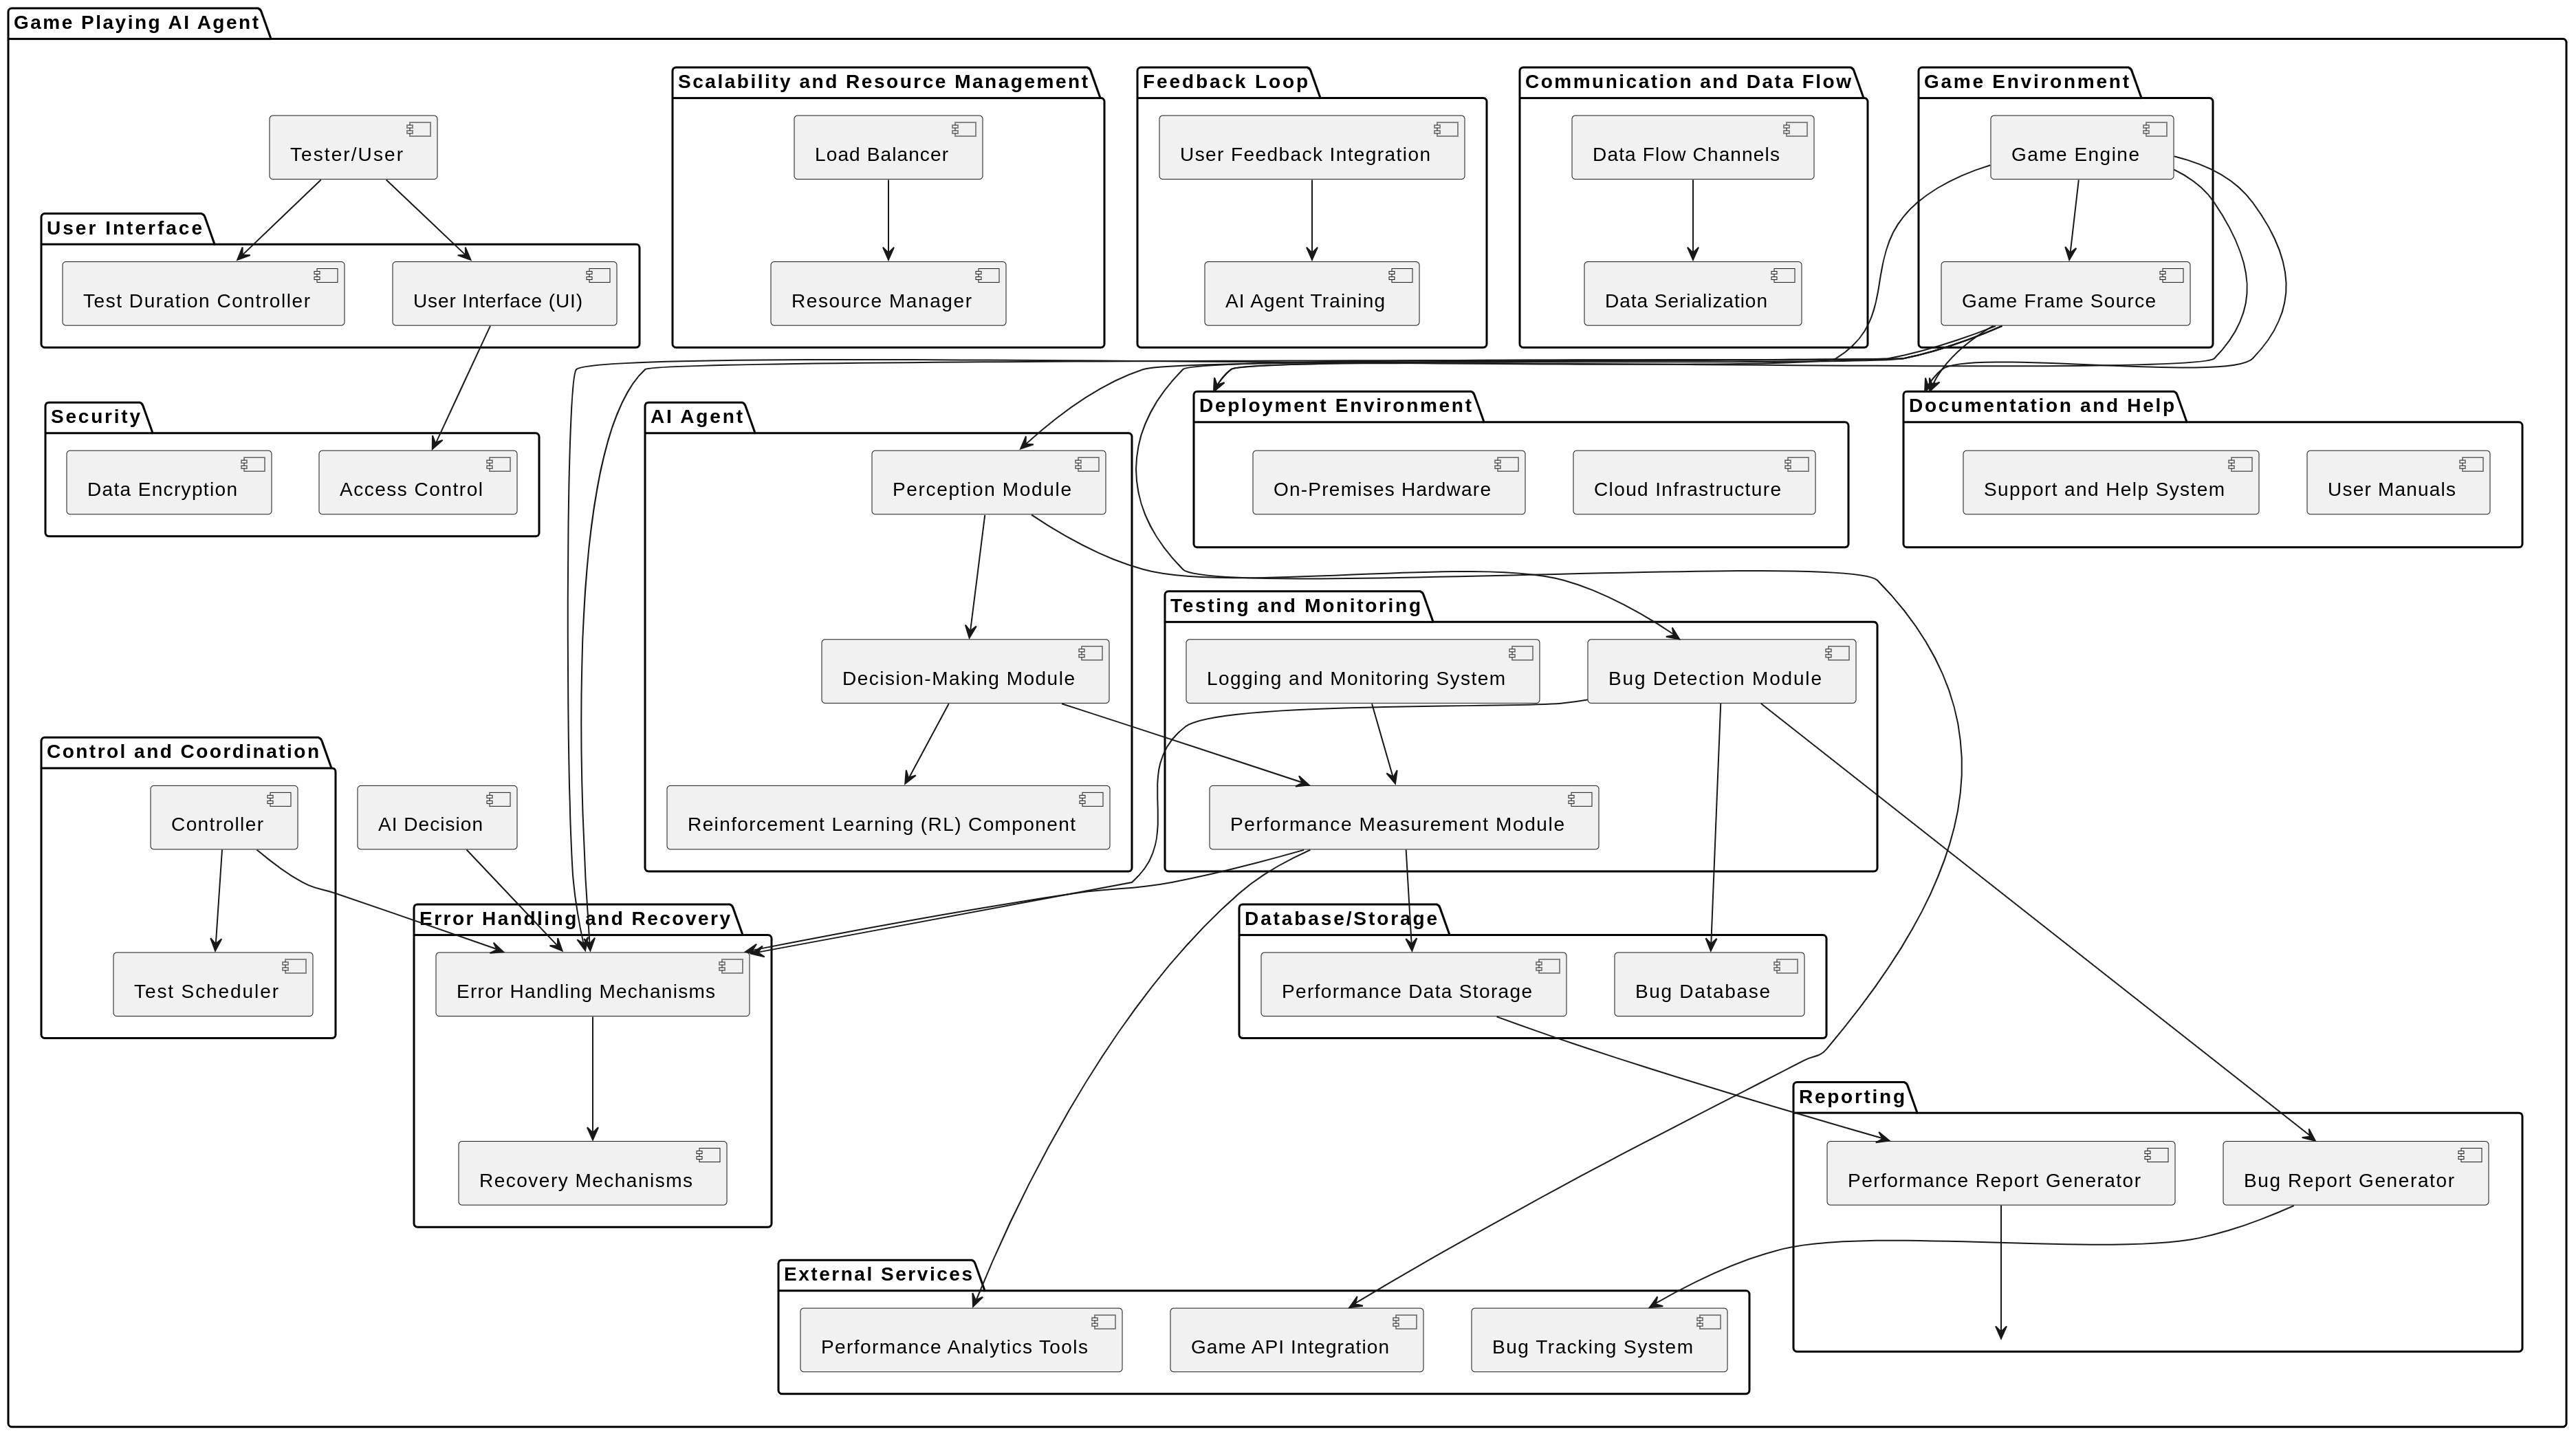
\includegraphics[width=\textwidth]{images/[1.0] sys arch.png}
% %         \caption{A detailed system flow diagram for an AI agent for game testing and automation}
% %         \label{fig:sysFlow}
% %     \end{figure}


\end{document}